
La modulation LoRa en tant que telle ne comprend pas d'aspect lié à la sécurité, car il ne s'agit que de la couche 1 du modèle OSI. La sécurité est gérée par les couches supérieures, ce qui relève du protocole que l'utilisateur souhaite appliquer au-dessus de la modulation. Cette section sécurité se concentre principalement sur le mode OTAA pour l'enregistrement sur un réseau. Celui-ci est considéré comme étant le plus sûr et le mieux adapté à des dispositifs LoRaWAN \cite{ttnvideos_security:online}\cite{LoRaSecu3:online}.\\


Le 11 octobre 2017, la LoRa Alliance a dévoilé la version définitive du protocole LoRaWAN 1.1. Les explications prodiguées dans les sous-sections qui suivent décrivent la version 1.0.2 de LoRaWAN. Peu d'opérateurs proposent un support pour la spécification 1.1. Par exemple, le réseau The Things Network a pour objectif d'apporter un support uniquement pour avril ou mai 2018. Le module LoRaWAN choisi n'est actuellement pas encore compatible avec cette dernière version. Toutefois, la mise à jour des périphériques ne nécessite qu'une mise à niveau logicielle et non matérielle. Un résumé des nouveautés de LoRaWAN 1.1 est proposé en \cref{sec-security_lorawan_1_1}.\\


Le 23 mars 2016, la société MWR InfoSecurity\footnote{\url{https://www.mwrinfosecurity.com/}} spécialisée dans la recherche et les conseils en sécurité informatique a publié un \textit{whitepaper} sur la sécurité d'un réseau LoRa. Le document est intitulé \textit{LoRa Security: Building a secure LoRa solution} et écrit par Robert Miller \cite{LoRaSecu3:online}. Les explications du présent chapitre ont été en partie reprises de ce \textit{whitepaper}, lequel contient un résumé des points essentiels présentés dans la spécification LoRaWAN\footnote{\url{https://www.lora-alliance.org/lorawan-for-developers}}.


\subsection{Rejoindre un réseau à l'aide d'OTAA}
\label{sec-security_lorawan_join}


La structure des paquets LoRaWAN a été présentée en \cref{sec-protocols_lorawan}. Il est important d'avoir en tête les différents champs de ces paquets pour comprendre la façon dont la sécurité est appliquée aux messages LoRaWAN.

\begin{figure}[ht!]
    \centering
    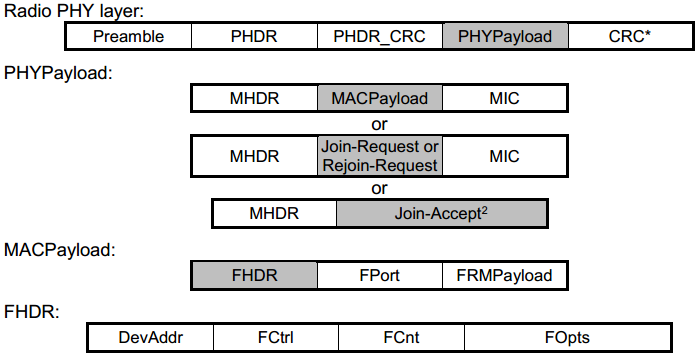
\includegraphics[width=0.8\textwidth]{Figures/Protocols/LoRaWAN/lorawan_mac_format_packets.png}
    \caption{Format des messages du protocole LoRaWAN}
    \label{fig-lorawan_mac_format_packets2}
\end{figure}

Chaque périphérique du réseau est déployé avec une \texttt{AppKey} et une \texttt{App EUI}. Cette première clé est indispensable lors de la procédure raccordement au réseau LoRaWAN pour authentifier le périphérique. L'\texttt{App EUI} est un identifiant qui est normalement unique pour l'utilisateur du périphérique et qui permet de déterminer à quelle application ce périphérique appartient. 
Pour initialiser cette procédure, le périphérique construit un message de type \texttt{Join Request} (cf. \cref{fig-lorawan_mac_format_packets2}) composé de l'\texttt{App EUI} de son \texttt{Dev EUI} de même que d'une valeur générée aléatoirement sur 2 bytes nommé DevNonce \cite{LoRaSecu3:online}. Le \texttt{Dev EUI} est l'identifiant unique du périphérique. Ces trois éléments sont ensuite signés à l'aide d'une valeur sur 4 bytes nommée \textit{Message Integrity Code} (MIC) et calculée comme suit :

\begin{tcolorbox}[top=-3mm, bottom=-3mm, left=0mm, right=0mm, enhanced, breakable, colback=LightGray, colframe=DarkGray, colbacktitle=DarkGray]
\begin{minted}[bgcolor=LightGray,fontsize=\footnotesize,breaklines]{python}
mac=aes128_cmac(AppKey, MHDR | AppEUI | DevEUI | DevNonce)
MIC = mac[0..3]
\end{minted}
\end{tcolorbox}


A la réception du message, le \textit{Network Server} détecte qu'il s'agit là d'un \textit{Join Request} et transfère la demande au \textit{Join Server} couplé à une valeur aléatoire (\textit{AppNonce}) qui sera utilisée pour la génération des clés. Le \textit{Join Server}vérifie les informations reçues afin de déterminer si le périphérique est ou non autorisé à rejoindre le réseau, puis il recalcule le MIC de son côté afin de s'assurer que le message n'a pas pu être altéré par une tierce personne. Si tout est validé, le \textit{Join Server} informe le \textit{Network Server} qu'une réponse de type \textit{Join Accept} doit être transmisse au périphérique. Cette réponse contient l'AppNonce précédemment généré par le \textit{Network Server}. Avec toutes ces informations, le serveur peut générer les deux clés de sessions (\textit{Network Session Key} et \textit{Application Session Key}) :

\begin{tcolorbox}[top=-3mm, bottom=-3mm, left=0mm, right=0mm, enhanced, breakable, colback=LightGray, colframe=DarkGray, colbacktitle=DarkGray]
\begin{minted}[bgcolor=LightGray,fontsize=\footnotesize,breaklines]{python}
NwkSKey = aes128_encrypt(AppKey, 0x01 | AppNonce | NetID | DevNonce | pad16)
AppSKey = aes128_encrypt(AppKey, 0x02 | AppNonce | NetID | DevNonce | pad16)
\end{minted}
\end{tcolorbox}

Le \textit{Join Accept} contient également les informations concernant les délais RF (RxDelay), le \textit{Dev Address} et la liste des canaux à utiliser (CFList). Un MIC doit être généré pour être ajouté au paquet de réponse :

\begin{tcolorbox}[top=-3mm, bottom=-3mm, left=0mm, right=0mm, enhanced, breakable, colback=LightGray, colframe=DarkGray, colbacktitle=DarkGray]
\begin{minted}[bgcolor=LightGray,fontsize=\footnotesize,breaklines]{python}
mac = aes128_cmac(AppKey, MHDR | AppNonce | NetID | DevAddr | RFU | RxDelay | CFList)
MIC = mac[0..3]
\end{minted}
\end{tcolorbox}

Les données sont retournées en utilisant l'\textit{AppKey} pour le chiffrement. A réception du paquet, le n\oe ud déchiffre les données et calcule à son tour les clés \textit{Network Session Key} et \textit{Application Session Key}. Ces deux clés sont maintenant utilisées pour chiffrer toutes les nouvelles données transmisses sur le réseau. La première pour les paquets qui sont envoyés sur le port 0 (\textit{Network Server}); la deuxième est quant à elle utilisée pour les données sur le port 1 à 223 impliquant l'\textit{Application Server}.

% La \cref{fig-keys_management_lorawan} démontre où les différentes clés de chiffrement sont présentes après qu'un périphérique aille rejoint un réseau en mode OTAA.

% \begin{figure}[ht!]
%     \centering
%     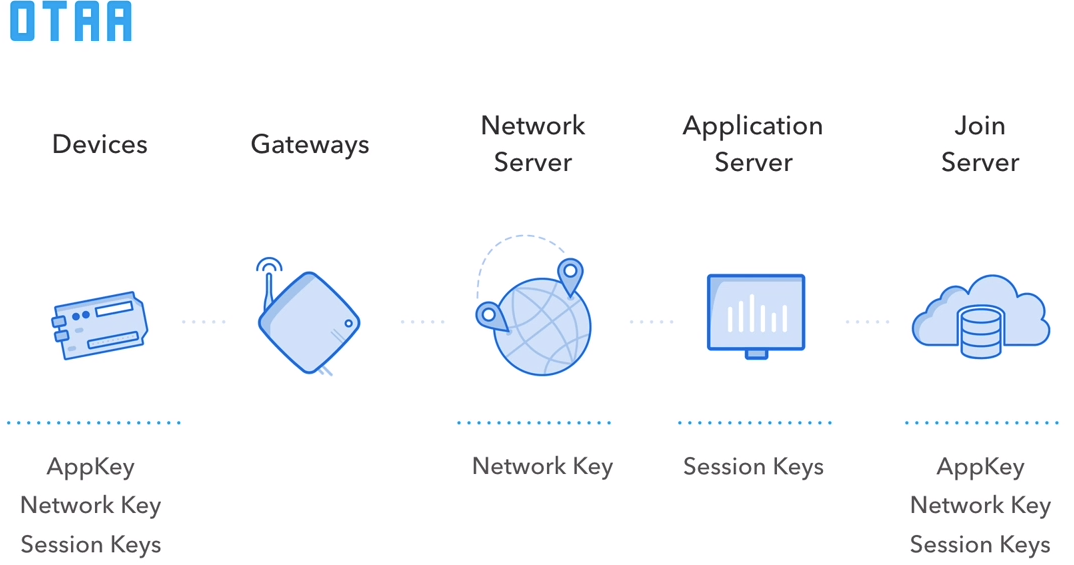
\includegraphics[width=0.8\textwidth]{Figures/Security/LoRaWAN/keys_management_lorawan.png}
%     \caption{Stockage des clés sur les différents composants d'une infrastructure LoRaWAN}
%     \label{fig-keys_management_lorawan}
% \end{figure}

\subsection{Protection des données}

Une fois un réseau LoRaWAN rejoint, toutes les données sont chiffrées en utilisant les deux clés de sessions.

\subsubsection{Chiffrement des données}

Le chiffrement des messages utilise AES-128\footnote{\url{https://en.wikipedia.org/wiki/Advanced_Encryption_Standard}} en \textit{Counter mode} (CTR) \cite{LoRaSecu3:online}. Une composante importante de la sécurité LoRaWAN réside dans les compteurs de messages \textit{uplink} (FCntUp) et \textit{downlink} (FCntDown) maintenus par le périphérique et le Network Serveur. Cette technique évite ainsi la possibilité de faire du \textit{replay attack}\footnote{\url{https://en.wikipedia.org/wiki/Replay_attack}} sur en copiant l'intégralité d'un paquet. 
Pour le chiffrement et le déchiffrement, un \textit{keystream} S est généré à l'aide des informations suivantes :

\begin{tcolorbox}[top=-3mm, bottom=-3mm, left=0mm, right=0mm, enhanced, breakable, colback=LightGray, colframe=DarkGray, colbacktitle=DarkGray]
\begin{minted}[bgcolor=LightGray,fontsize=\footnotesize,breaklines]{python}
i = 1..k where
k = ceil(len(FRMPayload) / 16)
Ai = (0x01 | (0x00 * 4) | Dir | DevAddr | FCntUp or FCntDown | 0x00 | i)
Si = aes128_encrypt(K,Ai), for i = 1..k
S = S1|S2|..|Sk
\end{minted}
\end{tcolorbox}

Une opération XOR est ensuite appliquée sur le champ \texttt{FRMPayload} avec le \textit{keystream} S pour chiffrer ou déchiffrer les données. Certaines données telles que le \texttt{FPort} ou \texttt{FCntUp} sont envoyées en clair.

\subsubsection{Signature des messages}

Dans le champ \textit{MAC Payload} (cf. \cref{fig-lorawan_mac_format_packets2}), les données sont singées afin d'éviter des modifications du \textit{cipher-text} ou d'autres valeurs comme le Dev Addr, FCnt ou FCntDown. De nouveau un champ MIC est utilisé comme signature :

\begin{tcolorbox}[top=-3mm, bottom=-3mm, left=0mm, right=0mm, enhanced, breakable, colback=LightGray, colframe=DarkGray, colbacktitle=DarkGray]
\begin{minted}[bgcolor=LightGray,fontsize=\footnotesize,breaklines]{python}
Msg = MHDR | FHDR | FPort | FRMPayload
B0 = (0x49 | 4*0x00 | Dir | DevAddr | FCntUp or FCntDown | 0x00 | len(msg) )
mac = aes128_cmac(NwkSKey, B0 | msg)
MIC = mac[0..3]
\end{minted}
\end{tcolorbox}


\subsubsection{Infrastructure des opérateurs LoRaWAN}
\label{sec-security_lorawan_providers}


L'architecture LoRaWAN a déjà été abordée en \cref{sec-protocols_lorawan_architecture}, avec la description des cinq composants principaux (périphérique, \textit{gateway}, \textit{Network Server}, \textit{Join Server} et \textit{Application Server}). \\
%Le stockage des clés sur les différents éléments du réseau est visible sur la \cref{fig-keys_management_lorawan}.\\

\begin{figure}[ht!]
    \centering
    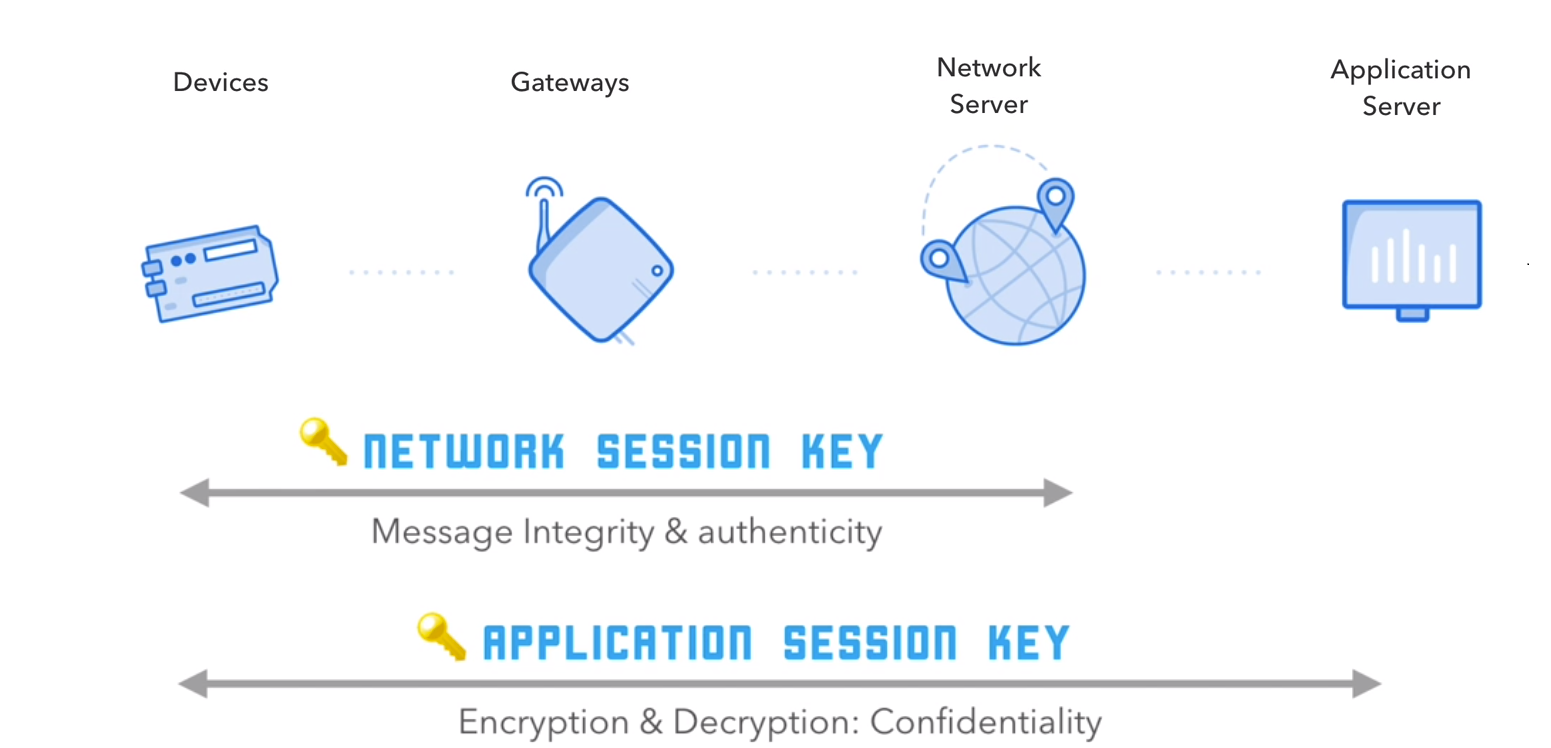
\includegraphics[width=0.85\textwidth]{Figures/Security/LoRaWAN/by_design_keys.PNG}
    \caption{Infrastructure d'un réseau LoRaWAN comme imaginée dans la spécification}
    \label{fig-by_design_keys}
\end{figure}

Le schéma de la \cref{fig-by_design_keys} expose l'utilisation des clés dans un réseau LoRaWAN. L'infrastructure y étant illustrée affiche une configuration pensée dans la spécification LoRaWAN: une séparation entre le \textit{Network Server} et l'\textit{Application Server}. \\

La réalité est quelque peu différente de cette implémentation. En effet, la plupart des fournisseurs de réseau LoRaWAN (The Things Network, Swisscom, Loriot, etc.) n'offrent pas la possibilité de séparer ces deux entités. L'architecture pratiquée par ces opérateurs est visible sur la \cref{fig-in_practice_keys}. L'opérateur possède les deux serveurs et fournit un accès au données au travers d'API propres à chacun. Cette architecture présente une problématique pour la sécurité des données. En effet, l'opérateur a à sa disposition la clé la plus importante, l'AppKey. Avec celle-ci, il doit générer la Network Session Key, indispensable à l'opérateur, et l'Application Session Key pour déchiffrer les données fournies à l'utilisateur. 
La plupart des opérateurs ont choisi cette approche puisque les clients ne souhaitent pas nécessairement mettre en place un \textit{Application Server} et un \textit{Join Server} en interne. Le SmartCanton a quant à lui décidé d'utiliser cette approche afin de garantir une sécurité et une maitrise totale sur les données tout en utilisant les infrastructures d'un opérateur existant pour le transport des paquets (cf. \cref{sec-smartcanton_security}).


\begin{figure}[ht!]
    \centering
    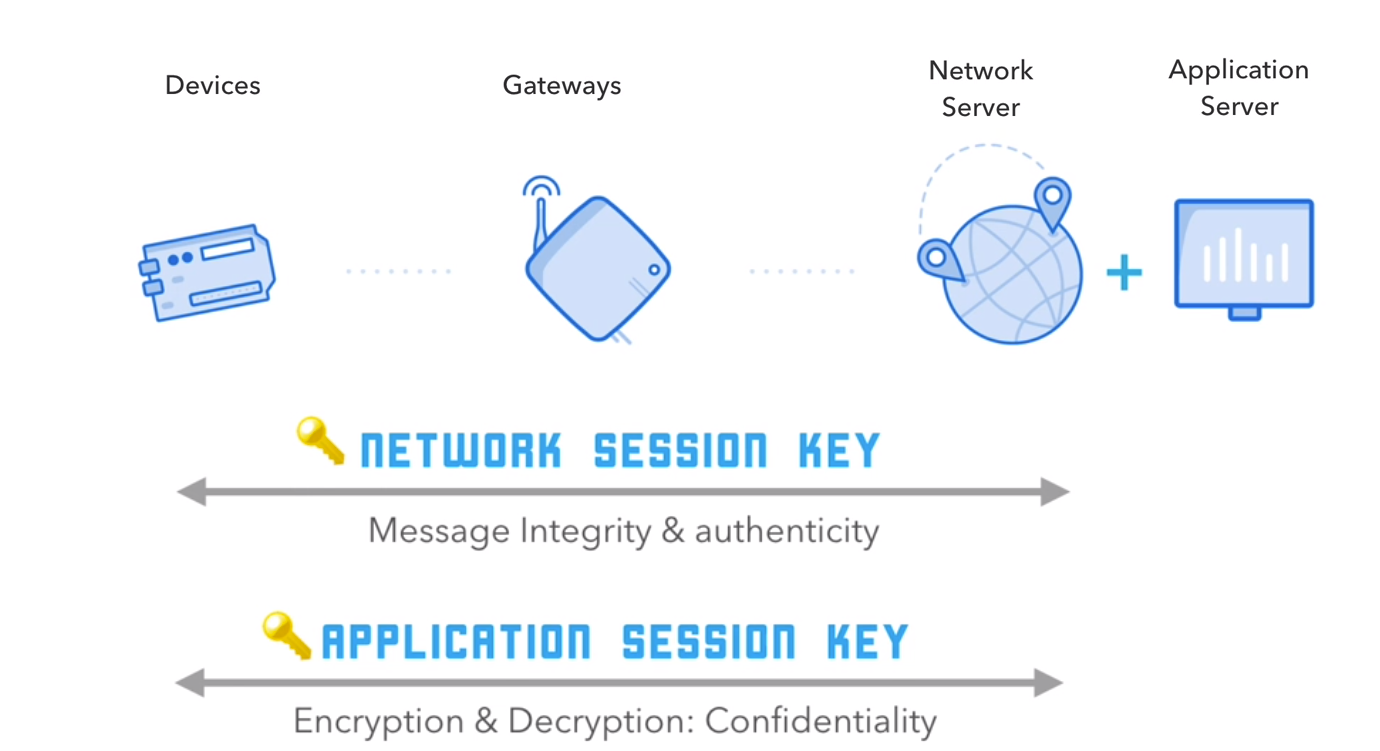
\includegraphics[width=0.85\textwidth]{Figures/Security/LoRaWAN/in_practice_keys.PNG}
    \caption{Infrastructure d'un réseau LoRaWAN réellement implémenté avec les opérateurs du marché}
    \label{fig-in_practice_keys}
\end{figure}



% ---------------------------------------------------------------------------------------
\subsection{LoRaWAN spécification 1.1}
\label{sec-security_lorawan_1_1}
% ---------------------------------------------------------------------------------------

La spécification LoRaWAN 1.1 apporte de nouvelles améliorations dans le domaine de la sécurité avec l'ajout de nouveaux concepts et des changements de mécanismes \cite{lorawan1_1_video:online}. Voici un résumé des changements principaux :
\begin{itemize}
    \item le compteur du nombre de paquets envoyés doit être stocké dans une mémoire non volatile et le même compteur ne peut pas être utilisable dans une même session. Un périphérique ABP ne peut ainsi plus être remis à zéro;
    
    \item DevNonce et JoinNonce (précédemment nommé AppNonce) ne sont plus aléatoire. Ce sont maintenant des valeurs incrémentales qui ne peuvent être utilisées qu'une seule fois et doivent être stockées en mémoire non volatile sur le périphérique;
    
    \item compteurs de message sur 32 bits (il s'agissait précédemment d'une recommandation, la version 16 bits était autorisée);
    
    \item deux compteurs de messages \textit{downlink} séparés; un pour le réseau (NFCntDown), l'autre pour l'application (AFCntDown);
    
    \item le compteur d'\textit{uplink} (FCntUp) est maintenant utilisé pour générer le MIC de l'\textit{acknowledge}.
    
\end{itemize}

Tous les périphériques doivent obligatoirement avoir la possibilité de stocker en mémoire non volatile les différentes informations. C'est la seule obligation matérielle impérative sur les périphériques 1.1. 

\begin{figure}[ht!]
    \centering
    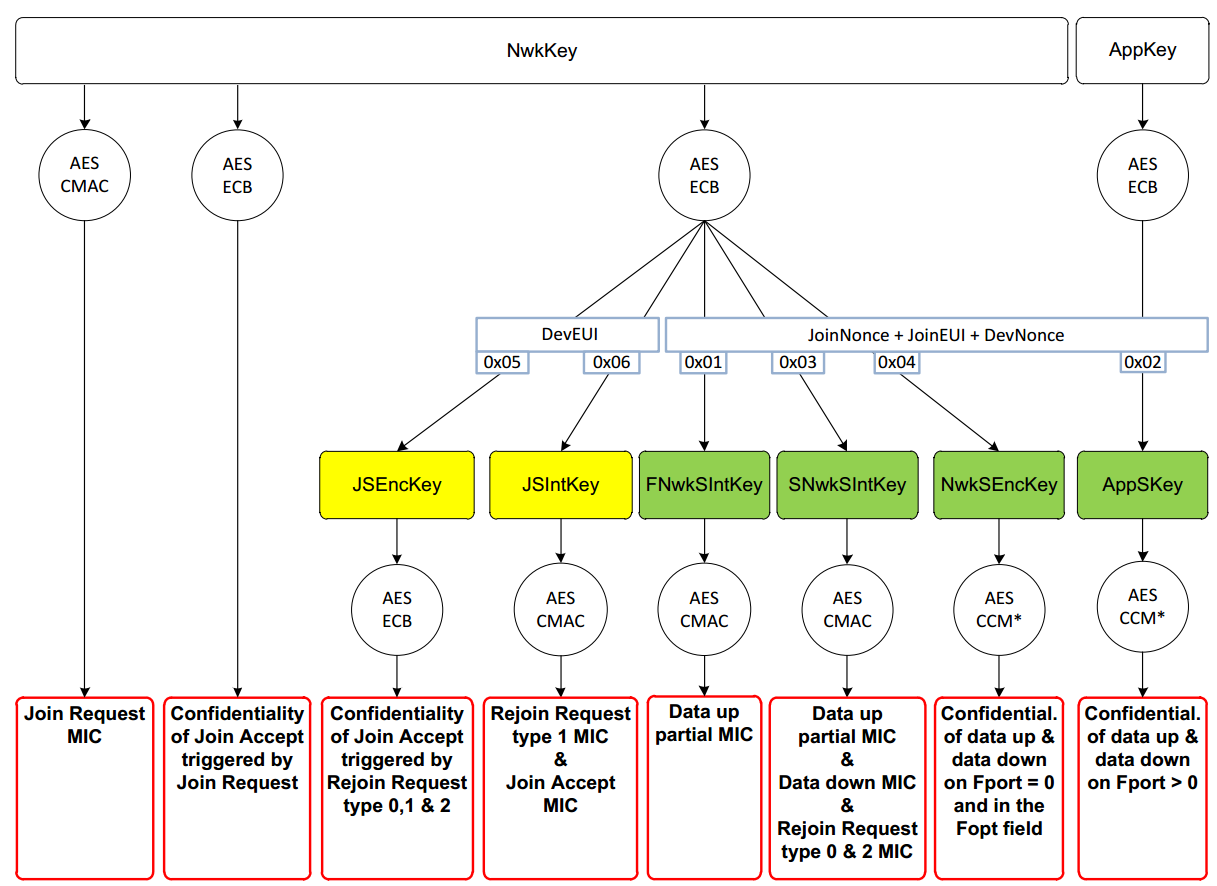
\includegraphics[width=1.0\textwidth]{Figures/Security/LoRaWAN/lorawan1_1_keys.PNG}
    \caption{Clés utilisées dans un réseau LoRaWAN avec la nouvelle spécification 1.1}
    \label{fig-lorawan1_1_keys}
\end{figure}

Le changement le plus important de la spécification 1.1 est l'introduction d'un nouveau secret partagé, nommé Network Key (\textbf{NwkKey}). Cette clé est utilisée pour créer trois nouvelles clés : 
\begin{enumerate}
    \item NwkSEncKey : clé utilisée pour chiffrer les commandes MAC;
    \item SNwkSIntKey : utilisée par un \textit{Serving Network Server} pour le calcul de la première moitié du MIC;
    \item FNwkSIntKey : utilisée par le \textit{Forwarding Network Server} pour le calcul de l'autre moitié du MIC.
\end{enumerate}

Une meilleure vue d'ensemble de toutes les clés et leur utilité est visible à l'aide de la \cref{fig-lorawan1_1_keys}. Si un périphérique 1.1 souhaite rejoindre un réseau gouverné par un Network Serveur 1.0, toutes les clés seront calculées à l'aide de la NwkKey. Les clés de sessions seront identiques et le périphérique n'utilisera plus sa AppKey. \\


Conjointement avec la parution de la spécification LoRaWAN 1.1, une nouvelle spécification pour la \textit{backend} des réseaux LoRaWAN nommée \textit{LoRaWAN Backend Interfaces 1.0 Specification} est disponible \cite{loraalli46:online}. Les informations de celles-ci affectent principalement les opérateurs de réseau LoRaWAN.

% ---------------------------------------------------------------------------------------
\subsection{Vulnérabilités et recommandations de sécurité}
\label{sec-security_lorawan_recommendatiions}
% ---------------------------------------------------------------------------------------

Les sous-sections qui suivent proposent quelques recommandations aux vulnérabilités sur les réseaux LoRaWAN \cite{ttnvideos_security:online} \cite{LoRaSecu3:online}. La spécification 1.1 apporte de nouvelles améliorations, toutefois certaines recommandations restent d'actualités \cite{lorawan1_1_video:online}.  

\subsubsection{Infrastructure du réseau}

L'infrastructure des opérateurs d'un réseau LoRaWAN a été étudiée en \cref{sec-security_lorawan_providers}. Laquelle a permis d'exposer la problématique sur le contrôle des serveurs. La plupart des opérateurs offrent une infrastructure complète avec l'intégration des trois serveurs. Il existe deux solutions pour pallier à cette problématique : 
\begin{enumerate}
    \item Utiliser un opérateur autorisant la connexion avec un \textit{Join Server} et un \textit{Application Server} externe. Cette approche est visible sur la \cref{fig-recommendations_a_private_domain}. Il s'agit là d'une réelle séparation des données et du réseau, comme la spécification LoRaWAN l'a prévu.
    
\begin{figure}[ht!]
    \centering
    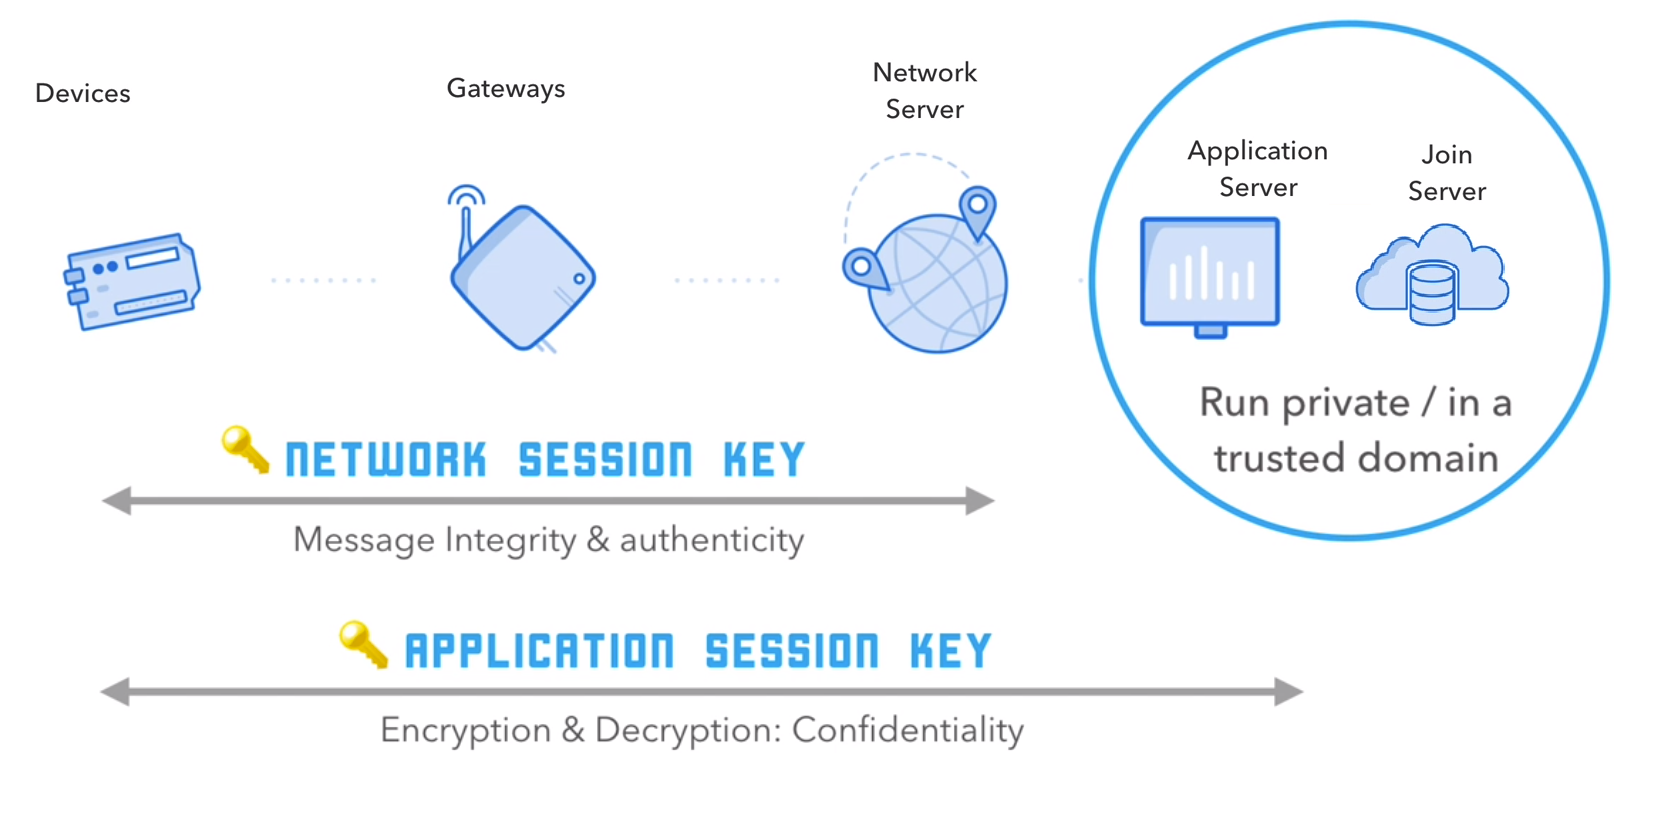
\includegraphics[width=0.9\textwidth]{Figures/Security/LoRaWAN/recommendations_a_private_domain.PNG}
    \caption{Recommandation pour l'implémentation d'une infrastructure LoRaWAN sécurisée}
    \label{fig-recommendations_a_private_domain}
\end{figure}

    \item Ajouter une nouvelle étape de chiffrement asymétrique, exploré sur la \cref{fig-recommendations_b_asymetric_crypto}. Lorsque cette option est utilisée, un opérateur de réseau LoRaWAN ne peut pas déchiffrer. Le déchiffrement peut ensuite être effectué par l'application finale qui se connecte au flux provenant de l'\textit{Application Server}.
    
\end{enumerate}




\begin{figure}[ht!]
    \centering
    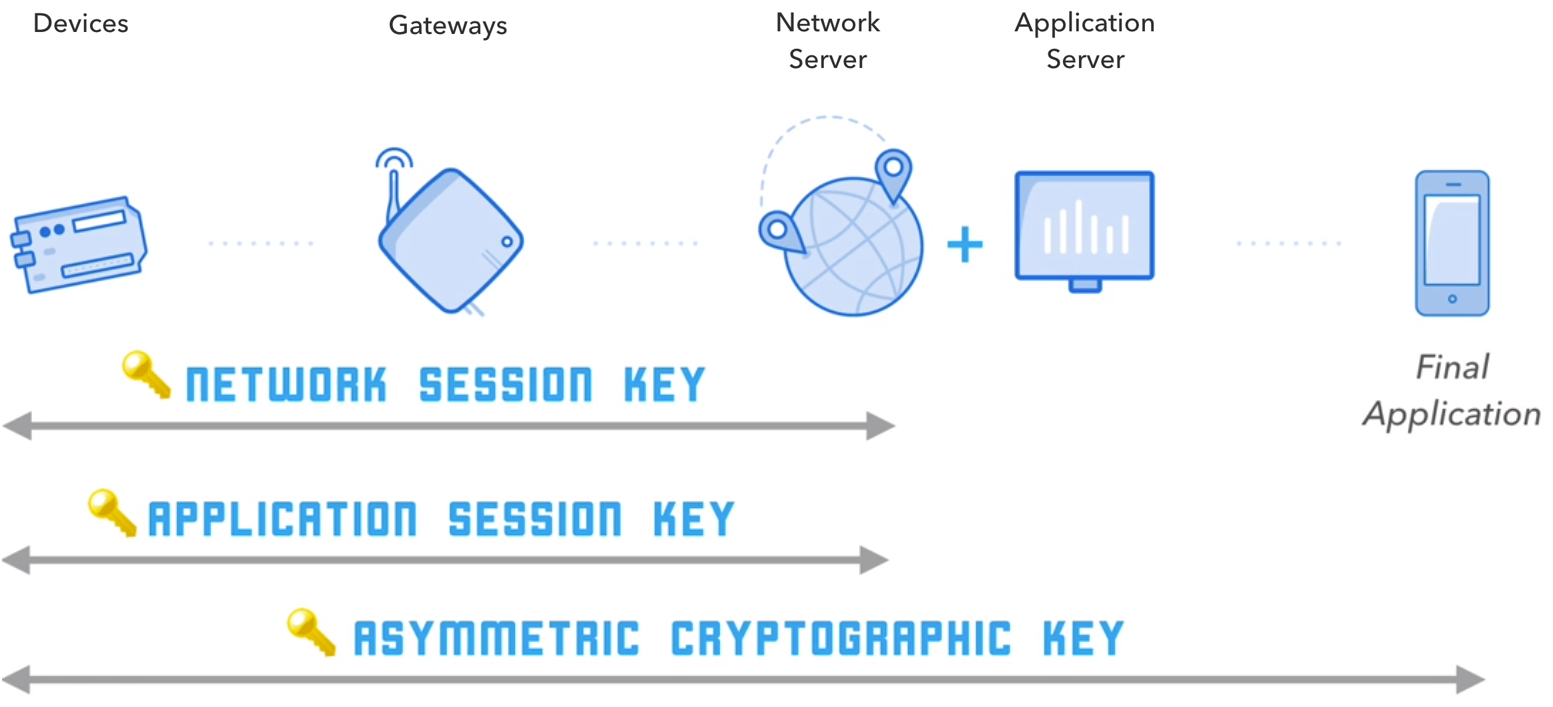
\includegraphics[width=0.9\textwidth]{Figures/Security/LoRaWAN/recommendations_b_asymetric_crypto.png}
    \caption{Clé asymétrique utilisée pour chiffrer les données}
    \label{fig-recommendations_b_asymetric_crypto}
\end{figure}


\subsubsection{Gestion des clés pour les périphériques}


Le mode de connexion le plus sécurisé est l'OTAA, car il ne nécessite que la connaissance d'un seul et unique secret partagé entre le \textit{Join Server} et le périphérique, l'AppKey. Lorsque l'une des deux clés de sessions est compromise, le périphérique peut être forcé à se joindre à nouveau au réseau et ainsi régénéré de nouvelles clés de session. La programmation des clés en ABP n'offre pas cette possibilité.\\

Un attaquant peut toujours récupérer des clés de chiffrements lorsqu'un accès direct au périphérique est possible. Par exemple, les attaques de type \textit{side channel analysis} qui consistent à mesurer la variation de courant ou la mesure des radiations électromagnétiques lorsque le \textit{transceiver} effectue le chiffrement AES pour déterminer la clé utilisée \cite{LoRaSecu3:online}. \\

Toutes les clés stockées sur les périphériques doivent être uniques. Il est possible d'assigner la même AppKey pour tous les périphériques, puisque l'identifiant unique du périphérique est le Dev EUI. Toutefois, ceci ne devrait jamais être le cas, car il suffit qu'un seul périphérique soit compromis pour que tous les périphériques d'un réseau doivent être reprogrammés. \\

La programmation des clés sur les périphériques ne doit pas se faire à l'aide de la même plage de fréquence que le LoRa \cite{ttnvideos_security:online}. Il est conseillé d'utiliser un nouveau type accès et ainsi appliquer un concept de \textit{out of the band}\footnote{\url{https://en.wikipedia.org/wiki/Out-of-band_data}} pour l'authentification, par exemple, en utilisant une technologie en 2.4 GHz. \\

Il est parfois possible d'envoyer un fichier binaire aux fabricants de cartes électroniques pour qu'ils programment directement les microcontrôleurs à la suite du montage des cartes électroniques \cite{ttnvideos_security:online}. Cette méthode est fortement déconseillée si le fabricant n'est pas de confiance. \\
 
Les clés ne doivent pas être stockées en tant que constantes dans le \textit{firmware} du microcontrôleur et la mémoire du microcontrôleur doit être sécurisée (cf. \cref{sec-security_hardware_protections} pour plus d'informations).


\subsubsection{Gestion des clés pour les serveurs}


Les serveurs doivent avoir accès aux différentes clés afin d'effectuer leurs tâches, mais celles-ci ne doivent être accessibles qu'à des personnes autorisées, que ce soit en lecture ou en écriture. \\

La génération de ces clés (cf. \cref{sec-security_lorawan_join}) doit être aléatoire, par exemple, en utilisant des \textit{true random number generators}.


\subsubsection{Compteur de paquets}

La vérification des compteurs de paquets doit être correctement effectuée par le \textit{Network Server}. Certains opérateurs allouent à l'utilisateur la possibilité de désactiver cette option pour effectuer des tests, mais ceci n'est pas acceptable lors d'une implémentation définitive. 


\subsubsection{Renouvellement des clés OTAA}


Lorsqu'un périphérique rejoint un réseau en OTAA, les clés de sessions générées sont utilisables indéfiniment \cite{ttnvideos_security:online}. Si le périphérique accepte les \textit{uplinks}, une commande applicative peut être envoyée pour demander au périphérique de relancer une nouvelle session à l'aide d'un \textit{join request}. Si les paquets \textit{downlink} ne sont pas implémentés, cette procédure peut être automatisée en local après l'envoi d'un nombre défini de paquets \textit{uplink}. Cette problématique a été corrigée avec le LoRaWAN 1.1 avec l'ajout de nouvelles commandes pour forcer un \textit{rejoin} du réseau en OTAA.


\subsubsection{Usurpation du microcontrôleur}




\begin{figure}[ht!]
    \centering
    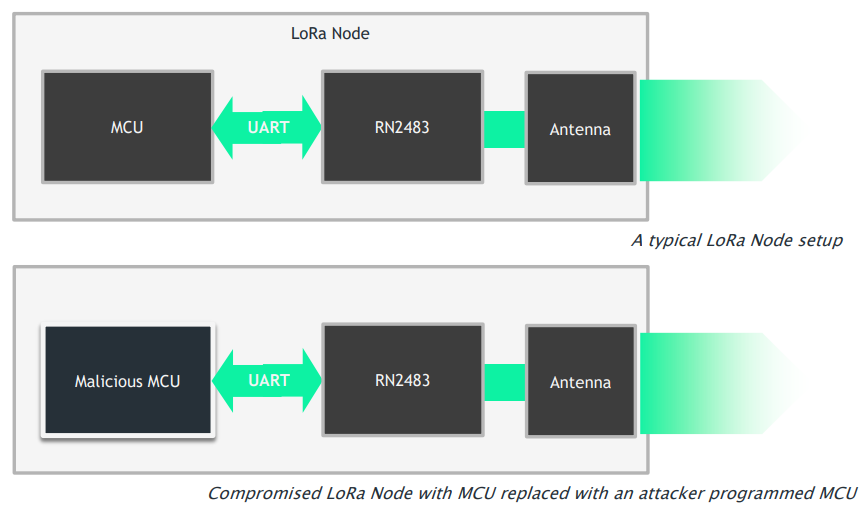
\includegraphics[width=0.65\textwidth]{Figures/Security/LoRaWAN/hardware_attack.png}
    \caption{Vulnérabilité des modules LoRaWAN avec le remplacement du microcontrôleur}
    \label{fig-hardware_attack}
\end{figure}

Lorsque l'attaquant dispose d'un accès direct sur le matériel, il lui est possible d'usurper le microcontrôleur principal communiquant. Par exemple, le RN2483 de Microchip \footnote{\url{https://www.microchip.com/wwwproducts/en/RN2483}} offre une interface UART pour la configuration. La \cref{fig-hardware_attack} expose la situation. Une solution pour pallier à ce type d'attaque consiste à utiliser un module qui ne peut pas être lu depuis l'extérieur. Une fois celui-ci programmé pour rejoindre un réseau, il sauvegarde dans sa mémoire non volatile les clés sans les redistribuer.
Il est possible de ne pas utiliser de coprocesseur LoRaWAN et d'implémenter la \textit{stack} LoRaWAN directement dans le processeur principal. On peut ainsi utiliser un circuit intégré radio de Semtech. Les inconvénients de ce type d'implémentation est la complexité logicielle ajoutée au processeur principal. En \cref{sec-security_hardware_protections} divers conseils relatifs au stockage des clés dans des mémoires non volatiles sont présentés.


\subsubsection{Accès aux \textit{gateways}}

Si un attaquant a accès à une \textit{gateway}, il ne peut pas accéder aux données, car celles-ci sont toujours chiffrées avec les différentes clés. Toutefois, il a la possibilité de la rendre inopérationnelle. L'attaquant peut également corrompre les données, mais dans ce cas, le \textit{Network Server} détectera cette corruption et les ignorera.
Les \textit{gateways} sont le plus souvent connectées à Internet pour créer le pont entre le protocole LoRaWAN et les serveurs. Il est important de les mettre à jour régulièrement, et tout particulièrement lorsqu’une vulnérabilité est découverte ou lorsqu'une nouvelle version du protocole est disponible. Cette mise à jour peut se faire en se déplaçant physiquement auprès de celle-ci ou à distance. La deuxième option est indispensable lorsqu'un grand parc de \textit{gateways} est maintenu. La connexion à celle-ci doit donc être sécurisée du mieux possible à l'aide mots de passe uniques pour chaque \textit{gateway} ou encore mieux, des clés d'authentifications (ex. clés SSH) gardées secrètes. 

